%!TEX root=../document.tex

\section{Ergebnisse}
\label{sec:Ergebnisse}
	
\subsection{Testen des Tutorialcodes}

\subsubsection{Buildautomation mit Ant}

Ant ist ein Bildautomationtool welches auf einer Datei namens build.xml
basiert. Hier werden viele Properties, Targets die das Programm umschreiben definiert. Die Properties sind insofern wichtig, da sie Informationen über den Classpath, Java Version, Binaries usw., enthalten.
Die angegebenen Targets können dann später nach dem builden mittels der Commandline wie folgt ausgeführt werden.

\begin{lstlisting}[caption=Ant Beispiel, language=bash]
	ant [target]
\end{lstlisting}

\subsubsection{Testen des simplen Tutorialcodes}

Bevor die Sockets die in dem Tutorial verwendet werden
funktionieren, muss man noch in der java.policy Datei ein paar Zeilen am Anfang wie folgt hinzufügen, da man sonst eine AccessControlException bei der Ausführung des engine Targets bekommt.

\begin{lstlisting}[caption=Bearbeiten von java.policy, language=bash]
	sudo vim /usr/lib/jvm/java-8-openjdk/jre/lib/security/java.policy
	
	// Inserted to grant all privileges
	grant codeBase "file:/home/sons/-" {
       	permission java.security.AllPermission;
	};
\end{lstlisting}

Um ein Projekt mit ant zu builden, geht man einfach per Commandline in den Projektordner mit dem Testcode.
Nun kann man mit den ant Targets den Server und Client starten (natürlich in seperaten Terminals). Engine entspricht hierbei dem Server, compute dem Client.

\begin{lstlisting}[caption=Builden mit ant, language=bash]
	cd ~/School/SYT/Syt_RMI/rmiTutorial
	ant 
	ant engine
	ant compute
\end{lstlisting}

% Codesegment einfügen
%\begin{lstlisting}[caption=P1 Struktured Text]
%			FuellstandT120:= S412;
%
%			V227:=1;
%			V224:=1;
%			V121:=1;
%			P220:=7;
%		\end{lstlisting}
%Listen erstellen
%\begin{itemize}
%	\item \textbf{ \"Ubungsteil 1:} 
%	\item \textbf{ \"Ubungsteil 2: } 
%\end{itemize}

%Bilder einfügen
%\begin{figure}[!h]
%	\begin{center}
%		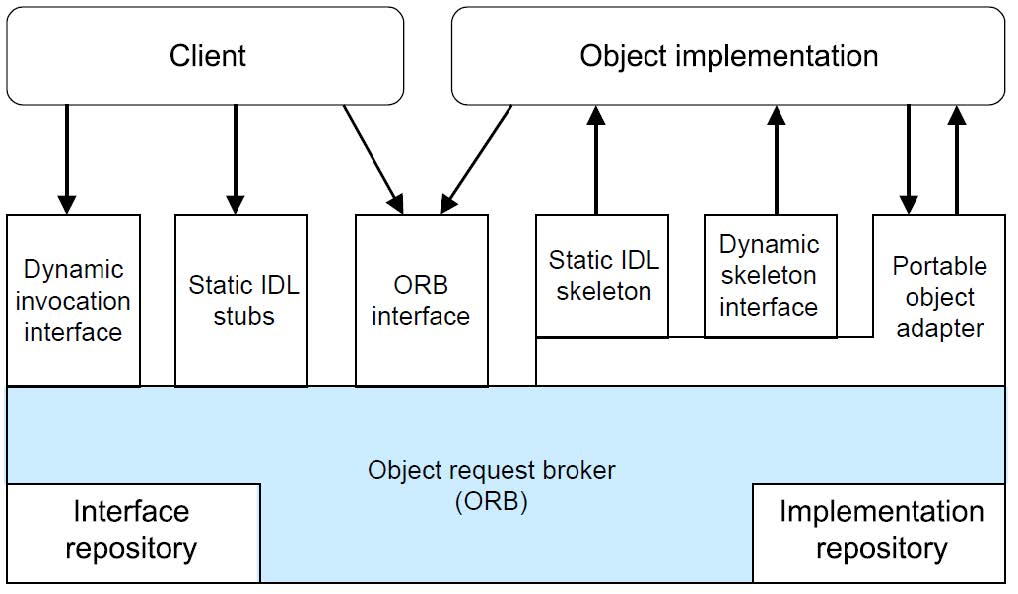
\includegraphics[width=0.5\linewidth]{images/corba.jpg}
%		\caption{Common Object-Request-Broker Architecture \cite{tanenbaum2007verteilte}}
%		\label{broker}
%	\end{center}
%\end{figure}
%

In Eclipse einbinden und dann in der Console mit 
ant im Projektordner das Projekt builden.
Wirft einen Fehler access denied Socket Permission
Lösung: im java.policy file die permissions anpassen.
Nun ant engine ausführen um den Server zu starten und
ant compute um sich pi zu berechnen.

\subsubsection{Testen des Command Patterns}

Um das vorbereitete Command Patter auszuprobieren, geht man wiederum mc cd in den Ornder mit dem jeweiligen Testcode und builded diesen mit dem ant Befehl.

\begin{lstlisting}[caption=Builden des Command Pattern Testcodes, language=bash]
	cd ~/School/SYT/Syt_RMI/rmiCommandPattern
	ant
\end{lstlisting}

Mittels der ant - Befehle "client" und "server", kann man nun die jeweils dem Namen entsprechenden Komponenten starten (in seperaten Terminalinstanzen versteht sich) .

\begin{lstlisting}[caption=Ausführen des Testcodes des Command Patterns, language=bash]
	ant server
	ant client
\end{lstlisting}

\subsection{Implementierung eines eigenen Command Patterns}

Aufgabe war es nun, ein eigenes Command Pattern zu erzeugen, welches am Server die Eulersche Zahl mit dem entsprechenden Algorithmus berechnet und das Ergebnis anschlie{\ss}end ausgibt.

\subsubsection{Implemetierung des Command Patterns}

Ein Command Pattern besteht aus zwei Interfaces, dem CommandExecutor und dem eigentlichen Command. Das Command Interface schreibt hier vor, 
dass es eine Methode execute geben muss, welche dann logischerwei{\ss}e vom CommandExecutor ausgeführt wird.
\begin{lstlisting}[caption=Command Interface, language=Java]
	public interface Command extends Serializable {
		public void execute();
	}
\end{lstlisting}

In diesem Beispiel heißt der CommandExecutor doSomethindService, ist aber gleich implementiert wie das standartmä{\ss}ige Interface.

\begin{lstlisting}[caption=Command Executor, language=Java]
	public interface DoSomethingService extends Remote {

	public void doSomething(Command c) throws RemoteException;
	
}
\end{lstlisting}

Dieses Interface wird nun in der Klasse ServerService konkret verwendet, um das Command auszuführen.

\begin{lstlisting}[caption=ServerService Klasse, language=Java]
	public class ServerService implements DoSomethingService {

	@Override
	public void doSomething(Command c) throws RemoteException {
		c.execute();

	}

}
\end{lstlisting}
\clearpage

\subsubsection{Implementierung eines Callbacks}

Damit der Server dem Client eine Rückmeldung nach der Berechnung schicken kann, hier etwa mit dem Ergebnis der Berechnung, muss man einen sogenannten Callback implementieren. Die Implemetierung passiert über ein Interface mit dem Namen Callback, welches 3 Methoden vorschreibt, nämlich :
\begin{itemize}
	\item \textbf{set} Setzt jenen Wert, welcher übetragen werden soll.
	\item \textbf{print} Schreibt den Wert in die Console.
	\item \textbf{receive} Gibt den Wert des Callbacks zurück. 
\end{itemize}

\begin{lstlisting}[caption=Interface für das Callback, language=Java]
	public interface Callback<T> extends Remote, Serializable {
	public void set(T argument) throws RemoteException;
	public void print() throws RemoteException;
	public T receive() throws RemoteException;
}

\end{lstlisting}

Nun habe ich dieses Interface auf eine Klasse CallResult angewandt, welche mit dem Typ Double arbeitet. Diese Klasse hat eine globale Variable result, welche von den 3 vorher erwähnten Methoden verwendet wird.

\begin{lstlisting}[caption=CallResult Klasse, language=Java]
	public class CallResult implements Callback<Double>, Serializable{

	private static Double result; 
	
	/**
	 * Set the value to be used by the other methods
	 */
	@Override
	public void set(Double result) throws RemoteException {
		// TODO Auto-generated method stub
		this.result = result;
	}

	/**
	 * Prints the result to the console
	 */
	@Override
	public void print() throws RemoteException {
		// TODO Auto-generated method stub
		System.out.println("The result is: "+result);
	}

	/**
	 * Receive the result
	 */
	@Override
	public Double receive() throws RemoteException {
		// TODO Auto-generated method stub
		return null;
	}

}
\end{lstlisting}
\clearpage

Um den Callback verwenden zu können, müssen noch zwei Zeilen Code in die Client Klasse hinzugefügt werden, welche das Callback Object exportieren. Hierbei wird aber nicht direkt in die Registry von RMI gespeichert, da sonst auch andere Clients auf den Callback zugreifen könnten, es soll aber nur dem Server möglich sein.

\begin{lstlisting}[caption=Implementierung des Callback am Client, language=Java]
			// Create a new callback
			Callback callback = new CallResult();
			
			// Export the callback
			Callback callbackStub = (Callback) UnicastRemoteObject.exportObject(callback,0);
\end{lstlisting}

\subsubsection{Implementierung des Euler-Algorithmus}

In EulerCalc, welches das Interface Calculation implementiert.

\begin{lstlisting}[caption=Calculation Interface, language=Java]
	public interface Calculation {

	public void calculate();
	public double getResult();
}
\end{lstlisting}

In calculate wird in der konkreten Klasse EulerCalc eine weitere Methode calcEuler aufgerufen, welche den Algorithmus zu Berechnung der eulerschen Zahl beinhaltet (diesers orientiet sich and er Summenformel welche die eulersche Zahl definiert). Diese sieht wie folgt aus:

\begin{lstlisting}[caption=Algorithms der eulerschen Zahl, language=Java]
	private void calcEuler(int digits){
		
		// Buffer for the current e
		double buffer = 1.0; 
		
		// current value of the fraction in the limes
		double currentNumber;
		
		// The factorial of the current fraction in the limes
		double factorial = 1.0;
		
		// This loop runs until the amount of digits the user
		// whiched for is reached
		for(int i=1; i < digits;i++){
			
			// Multiply the factorial with the counter, so it
			// behaves like a mathematical factorial
			factorial = factorial * i; 
			
			// By dividing 1 through the current factorial you
			// get the digit at count i for the number e
			currentNumber = 1 / factorial;
			
			// add the current number to the buffer
			buffer += currentNumber;
		}
		
		// Set global variable result to the value of buffer
		result = buffer;
	}
\end{lstlisting}

Mit getResult kann man schlie{\ss}lich auf das Ergebnis dieser Berechnung zurückgreifen.

\subsubsection{Implementieren des CalculationCommands}

Hier passiert eigentlich die ganze "Magie" des Callbacks und des Commands. Mittels zwei Parametern werden sowohl ein Callback, als auch ein Calculation Objekt übergeben und auf die Attribute der Klasse geschrieben. In der execute Methode wird nun das Ergebnis berechnet, und dieses dann mit set auf den Callback geschrieben und dann mit print an den Client gesendet. \\ 

Wieder in der Client Klasse man noch das Command aufrufen, mit dem voher gesetzen Callback und einem neuen EulerCalc Objekt als Parameter.

\begin{lstlisting}[caption=Aufrufen des Commandos, language=Java]
				Command calcEuler = new CalculationCommand(new EulerCalc(), callback);

\end{lstlisting}

\subsection{Darstellung in UML}

\subsection{Zeitaufzeichnung}





